% 2010 年广东卷理科第 18 题：半圆 AEC 与三棱锥 F-BED，含 Q、R。
% 来源 PDF：普通高考/2010/2010广东理.pdf，SHA-256 1c708f5a82d57782cd31357148f1dba05af44c63ffab0045cf301c88eb5d5fd7。
% 原页：第 2 页（A3 三栏）第 1 栏上部，书页码 594。
% 重绘依据：A、B、C、D 共线且 AB=BC=CD；半圆以 AC 为直径、E 为弧中点；
%   Q、R 分别在 FE、FB 上，FQ=2/3 FE、FR=2/3 FB；FB 为不可见棱，画虚线。
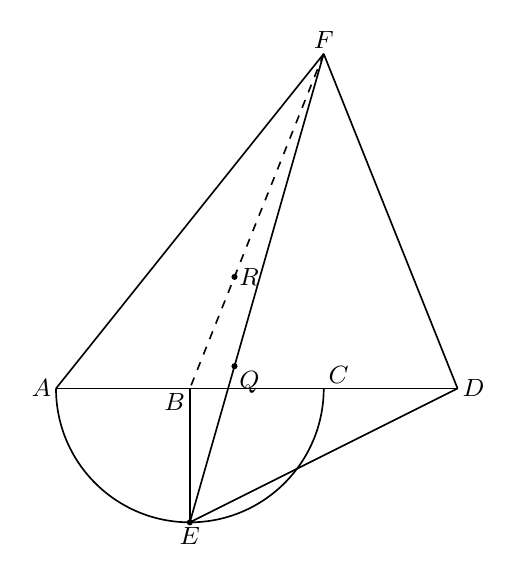
\begin{tikzpicture}[semithick, scale=0.85, every node/.style={inner sep=1.5pt, font=\small}]
  \coordinate (A) at (-2,0);
  \coordinate (B) at (0,0);
  \coordinate (C) at (2,0);
  \coordinate (D) at (4,0);
  \coordinate (E) at (0,-2);
  \coordinate (F) at (2,5);
  \coordinate (Q) at (0.667,0.333);
  \coordinate (R) at (0.667,1.667);

  \draw (A) -- (D);
  \draw (A) arc[start angle=180,end angle=360,radius=2];
  \draw (F) -- (A);
  \draw (F) -- (D);
  \draw (F) -- (E);
  \draw[dashed] (F) -- (B);
  \draw (E) -- (B);
  \draw (E) -- (D);

  \fill (E) circle (1.3pt);
  \fill (Q) circle (1.3pt);
  \fill (R) circle (1.3pt);
  \node[left] at (A) {$A$};
  \node[below left] at (B) {$B$};
  \node[above right] at (C) {$C$};
  \node[right] at (D) {$D$};
  \node[below] at (E) {$E$};
  \node[above] at (F) {$F$};
  \node[below right] at (Q) {$Q$};
  \node[right] at (R) {$R$};
\end{tikzpicture}
